\documentclass{llncs}
\usepackage[utf8]{inputenc}
\usepackage[T1]{fontenc}
\usepackage[final]{graphicx}
\usepackage{epstopdf}
\usepackage[labelsep=period]{caption}
\usepackage[hyphens]{url}
\usepackage{amssymb,amsmath,mathrsfs}
\usepackage[russian,english]{babel}
\usepackage{graphicx}
\usepackage{multicol}
\usepackage[ruled,vlined,linesnumbered,algosection,algo2e]{algorithm2e}
\usepackage{algorithm}
\usepackage[noend]{algorithmic}

\tolerance=1000
\hbadness=5000
\newcommand{\const}{\mathrm{const}}
\newcommand{\tsum}{\mathop{\textstyle\sum}\limits}
\newcommand{\tprod}{\mathop{\textstyle\prod}\limits}
\newcommand{\cov}{\mathop{\rm cov}\limits}
\newcommand{\Dir}{\mathop{\rm Dir}\nolimits}
\newcommand{\KL}{\mathop{\rm KL}\nolimits}
%\renewcommand{\geq}{\geqslant}
%\renewcommand{\leq}{\leqslant}
\newcommand{\eps}{\varepsilon}
\newcommand{\cond}{\mspace{3mu}{|}\mspace{3mu}}
\newcommand{\Loss}{\mathscr{L}}
\newcommand{\RR}{\mathbb{R}}
\newcommand{\cL}{\mathscr{L}}
\newcommand{\cP}{\mathscr{P}}
\SetKwFor{ForAll}{\textbf{for all}}{}{}

\begin{document}
%%Analysis of Images, Social Networks, and Texts
\title{
    BigARTM: Open Source Library for
    Regularized %Multimodal Online Parallel Distributed
    Topic Modeling
    of Large Text Collections
}
\author{
    Konstantin Vorontsov\inst{1,3}
    \and
    Oleksandr Frei\inst{2}
    \and
    Murat Apishev\inst{3}
    \and
    Peter Romov\inst{4}
}
\institute{
    Department of Intelligent Systems at Dorodnicyn Computing Centre of RAS,
    Moscow Institute of Physics and Technology,
    \email{voron@forecsys.ru}
    \and
    Schlumberger
    \email{...}
    \and
    Moscow State University,
    \email{...}
    \and
    Yandex
    \email{...}
}

\maketitle

\begin{abstract}
    BigARTM

\vspace{1em}
\textbf{Keywords:}
    probabilistic topic model,
    Probabilistic Latent Sematic Analysis,
    Latent Dirichlet Allocation,
    stochastic matrix factorization,
    regularization,
    EM-algorithm,
    BigARTM.
\end{abstract}

\section{Introduction}
\cite{hofmann99plsi}
\cite{blei03latent}
\cite{asuncion09smoothing}

\cite{voron14dan-eng}
\cite{voron14aist}
\cite{voron14mlj}

\section{Multimodal regularized topic model}
\label{sec:Multimodal}

multimodal LDA (mmLDA) and correspondence LDA (Corr-LDA)
\cite{blei03modeling}

Matching Words and Pictures, MoM-LDA
\cite{barnard03matching}

\cite{rubin12statistical}

\cite{virtanen12factorized}

\cite{roller13multimodal}


\section{Online topic modeling}
\label{sec:Online}

\cite{hoffman10online}

\cite{zhang13sparse}

\section{BigARTM architecture}
\label{sec:BigARTM}

\subsection{Algorithm}

\begin{algorithm}
\caption{Online EM-algorithm}
\label{fig:plsa_alg}
\begin{algorithmic}[1]
\STATE Initialize $\phi_{wt}$ for all $w \in W$ and $t \in T$;
\STATE $n_{wt} := 0$, $\tilde n_{wt} := 0$
\FORALL{batches $D_j$, j = 1,...,J}
    \STATE $\tilde n_{wt} := \tilde n_{wt} + ProcessBatch(D_j, \phi_{wt})$
    \IF{(synchronize)}
        \STATE $n_{wt} := Merge(n_{wt}, \tilde n_{dw})$;
        \STATE $r_{wt} := Regularize(n_{wt})$;
        %\STATE $n_t := \sum_{w \in W} max(0, n_{wt} + r_{wt})$;
        \STATE $\phi_{wt} := Normalize(n_{wt} + r_{wt})$;
        \STATE $\tilde n_{dw} := 0$;
    \ENDIF
\ENDFOR
\end{algorithmic}
\end{algorithm}

\begin{algorithm}
\caption{$ProcessBatch(D_j, \phi_{wt})$}
\label{fig:plsa_alg}
\begin{algorithmic}[1]
\REQUIRE Batch $D_j$, Matrix $\phi_{wt}$;
\ENSURE $n_{wt}$;
\STATE $n_{wt} := 0$ for all $w \in W$ and $t \in T$;
\FORALL{ $d \in D_j$}
	\STATE initialize $\theta_{td}$ for all $t \in T$;
	\REPEAT
		\STATE $Z_w := \sum_{t \in T} \phi_{wt} \theta_{td}$ for all $w \in d$;
		\STATE $\theta_{td} := \frac{1}{n_d} \sum_{w \in d} n_{dw} \phi_{wt} \theta_{td} / Z_w$
               for all $t \in T$;
	\UNTIL{$\theta_d$ converges};
	\STATE increment $\tilde n_{wt}$ by $n_{dw} \phi_{wt} \theta_{td} / Z_w$
           for all $w \in d$ and $t \in T$;
\ENDFOR
\end{algorithmic}
\end{algorithm}

\subsection{Concurrency}
BigARTM can utilize multiple CPU cores by processing several batches in parallel,
which follows the rule of expressing parallelism at the highest possible level.
A alternative would be to parallelize the $ProcessBatch(D_j, \phi_{wt})$ routine,
but keeping it simple has many obvious benefits --- single-threaded code is much easier to modify and optimize.

\begin{figure}[h!]
\begin{centering}
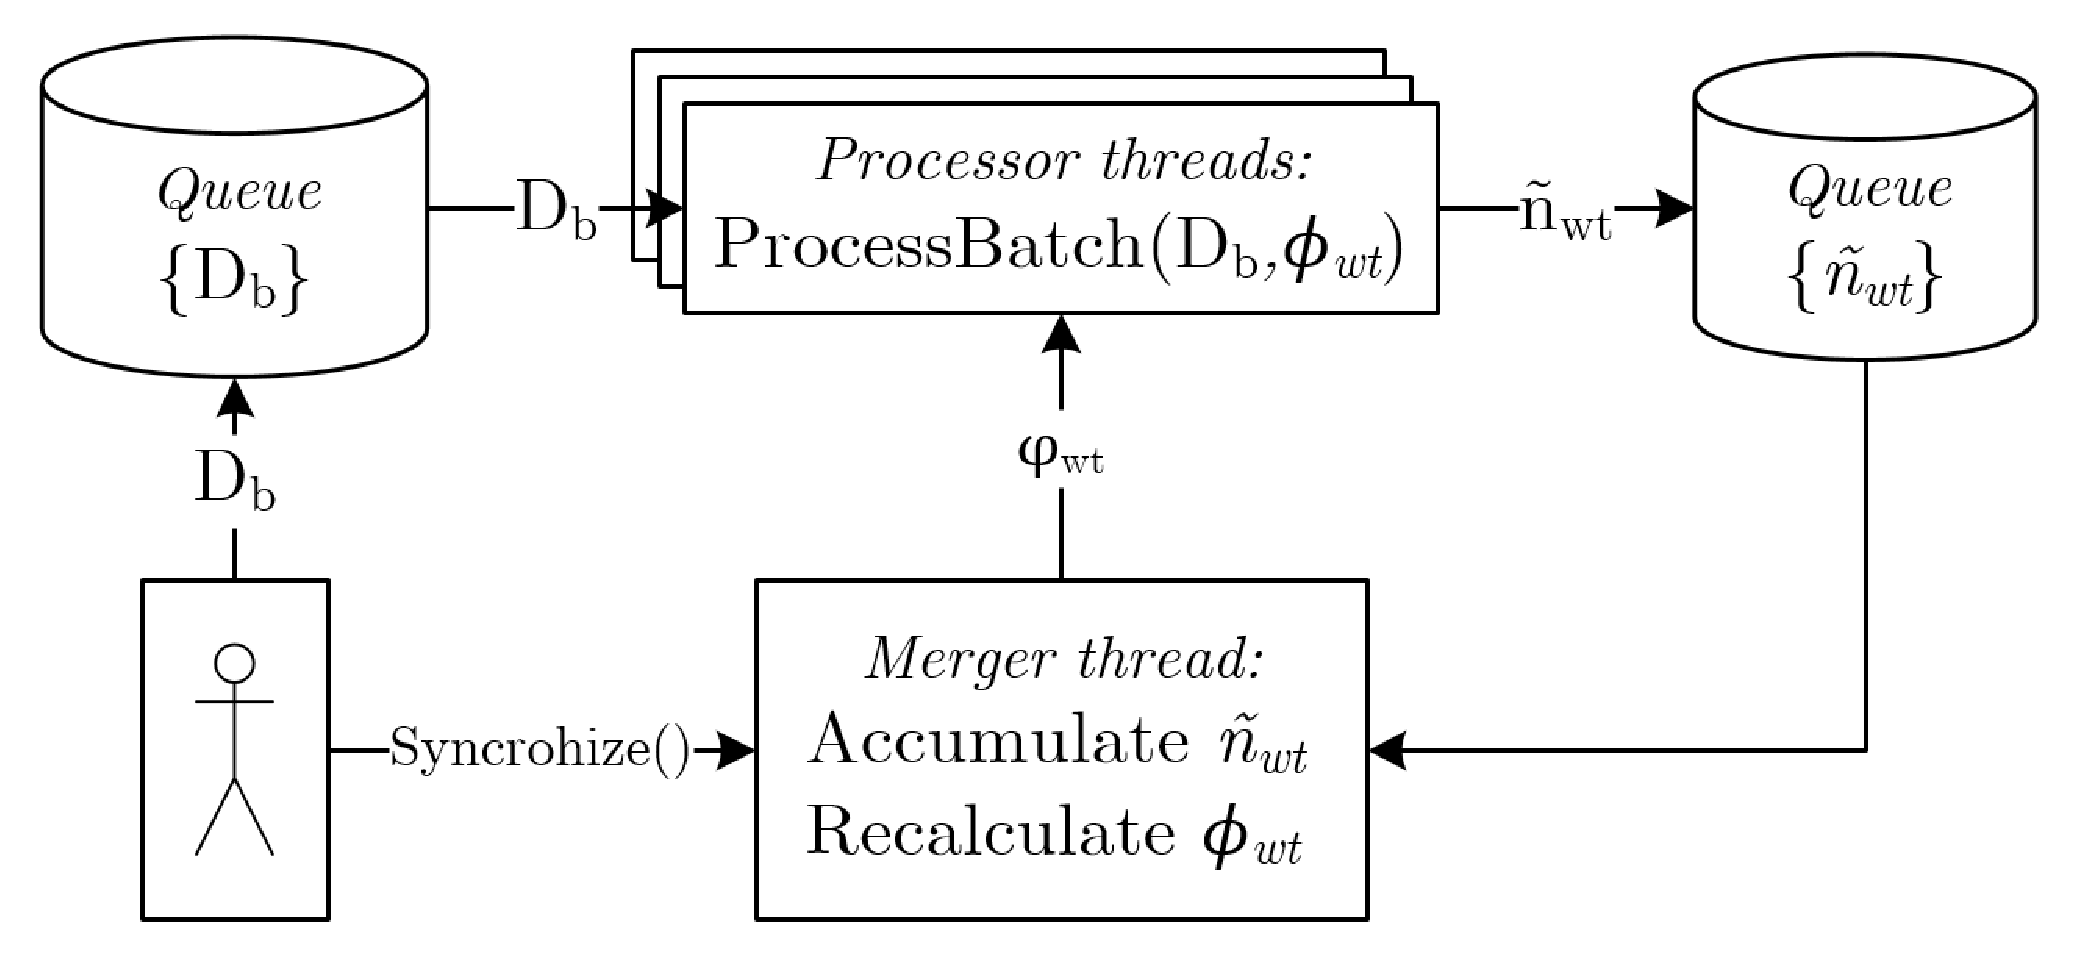
\includegraphics[height=48mm]{diagramm_artm_core.eps}
\caption{Diagram of key BigARTM components}
\label{fig:diagramm_artm_core}
\end{centering}
\end{figure}

Inputs and the outputs of $ProcessBatch$ routine are stored in two in-memory queues,
locked for push and pop operations with spin locks.
This approach does not add any noticeable synchronization overhead because
both queues only store smart pointers to the actual data objects,
so push and pop operations does not involve copying of real memory.

Smart pointers are also essential for handling of the $\phi_{wt}$ matrix.
This matrix is \emph{read} by all processors threads, and can be \emph{written} at any time by the merger thread.
To resolve this conflict we keep two copies of the $\phi_{wt}$ --- an \emph{active $\Phi$} and a \emph{background $\Phi$} matrices.
The active matrix is read-only, and is used by the processor threads.
The background matrix is being built in a background by the merger thread from $n_{wt}$ and $r_{wt}$ counters,
and once it is ready merger thread marks it as active.
Before processing a new batch the processor threads gets the current active matrix from the merger thread.
This object is passed via shared smart pointer to ensure that processor thread can keep ownership of the $\phi_{wt}$ matrix
until the batch is fully processed.

Having two copies of the $\Phi$ matrix is an obvious drawback of this solution.
An alternative would be to use atomic CPU instructions to read and write values of the $\Phi$ matrix.
Such operations are very efficient, but still come at a considerable synchronization cost
\footnote{http://stackoverflow.com/questions/2538070/atomic-operation-cost}.
Using them for all reads and writes of the $\Phi$ matrix would cause significant performance degradation for merger and processor threads.
Besides, an arbitrary overlap between reads and writes of the $\Phi$ matrix eliminates any possibility of producing a deterministic result.
The design with two copies of the $\Phi$ matrix give much more control over this
and in certain cases allows BigARTM to behave in a fully deterministic way.

The design with two $\Phi$ matrices only support a single merger thread,
and we believe it should cape with all $\hat n_{wt}$ updates coming from many threads.
This is a reasonable assumption because
$Merge$ routine takes only about $O(W * T)$ operations to execute, while
$ProcessBatch()$ takes $O(N_{nz} * T * I)$ operations,
where
$W$ is the size of the dictionary,
$N_{nz}$ is the number of non-zero entries in the batch,
$T$ is the number of topics,
and $I$ is the averate number of inner iterations in $ProcessBatch()$ routine.
$N_{nz} / W$ is typically 100 to 1000 (based on datasets in UCI Bag-Of-Words repository),
and $I$ is $10 \dots 20$, so the ratio safely exceeds the expected number of cores
(up to 32 physical CPU cores in modern workstations, and even 60 cores if we are talking about Intel Xeon Phi co-processors).

\subsection{Memory layout}

\subsection{Programming interface}

The core of BigARTM is written in C++, but we decided to wrap it into an ``extern C'' API.
This makes it very easy to consume BigARTM from almost any programming environment,
because there is always a way of calling ``extern C'' code
(ctypes module for Python, loadlibrary for Matlab, PInvoke for C\#, etc).








\section{Experiments}
\label{sec:Experiments}

\section{Conclusions}
\label{sec:Conclusions}

\bigskip
\subsubsection*{Acknowledgements.}
    The work was supported by~the Russian Foundation for Basic Research grants 14-07-00847, 14-07-00908,
    and by~Skolkovo Institute of Science and Technology (project 081-R).

%%%%%%%%%%%%%%%%%%%%%%%%%%%%%%%%%%%%%%%%%%%%%%%%%%%%%%%%%%%%%%%%%%%%%%%%%%%%
%\def\BibUrl#1.{\relax}
%\bibliographystyle{gost71sv}
\bibliographystyle{splncs}
\bibliography{MachLearn}
%%%%%%%%%%%%%%%%%%%%%%%%%%%%%%%%%%%%%%%%%%%%%%%%%%%%%%%%%%%%%%%%%%%%%%%%%%%%


\end{document}
